\section{Introduction}

These notes are personal (subjective) notes about different topics connected to
chromatography modelling. It is like an collage comprised from different
snippets theory snippets.

Some facts may be wrong, therefore please be critical during the usage of the
notes. Any caught mistakes and suggested corrections will be highly appreciated.

\section{Column characterization}
\subsection{Pore size distribution notes}

See Fabi article.

One of the key property of the packed chromatographic columns is its pore size
distribution (PSD). The packed column consists of porous spherical beads (we
assume those are rigid) squeezed together in a cylindrical shaped housing
conventionally called column.

When liquid (usually water solution) travels through such column any
dissolved particles enter and exit pores by means of diffusion, convection or
mass transfer. If we neglect any interaction of particles with the surface of
beads or work in non-binding conditions, particles that enter pores less often
or less deep will travel through the column faster. On the other hand particles
that can reach deep inside many of the pores will travel along the column
slower and thus reach the end of the column at latter time or volume.

Just as a side note, if the conditions are not perfectly non binding, then
exclusion, besides steric basis, may also arise due to: 
\begin{itemize}
    \item if one component is more strongly retained than
    other it will be unable to displace first component and thus won't be able to
        interact with surface.
    \item if component is charged with the same sign as the surface the
        particles will have difficulties entering pores due to Donnan effect.
\end{itemize}

Particle size as well as pore size both play major part in this size exclusion
process. Thus, in order to properly model flow of any particle (even the ones
that have strong interactions with the surface chemistry), having deep
knowledge about PSD is critical.

One way to experimentally determine PSD is to probe the column with
non-interacting particles of different but well known sizes. Very efficient and
well-behaved molecules that are often utilized in such column scrutinization
are Dextrans\footnote{Dextran is a complex branched glucan (polysaccharide
derived from the condensation of glucose), originally derived from wine.} 
of different sizes.

% TODO (ljeromel): Matic add table of dextrans.

For example Dextran-blue (mass of) is regularly utilized to determine
extraparticle volume void (extraparticle porosity).

Let us first define retention (elution) volume. Retention volume of a component 
is the volume after which the component It is measured from the point when
sample with the component is applied to the top of the column and to the point when that
specific component flows out of the bottom of the column. We will denote this
with $V_m$, $m$ as a probing molecule rather than c for component which would collide
with the column :).

Within the chromatographic column there are three characteristic volumes:

\begin{itemize}
    \item Total column volume $V_c$ - volume of the empty "glass" cylinder which is
        used as the column housing and into which we pack the resin beads. 
    \item Extra particle void volume $V_0$ - empty volume between the
        particles. It is the empty volume of the packed colum if particles
        wouldn't be porous (full beads).
    \item Intra particle void volume $V_{p}$ - empty volume within all beads.
\end{itemize}

The intra particle void volume $V_{p}$ is actually sum of all void volumes of
each individual bead, $V_{pi}$:

\[V_p = \sum_{i}^{N}V_{pi},\]

where $N$ is total number of particles within the column (usually this is not
known and almost impossible to determine).


\begin{figure}[h]
	\centering
    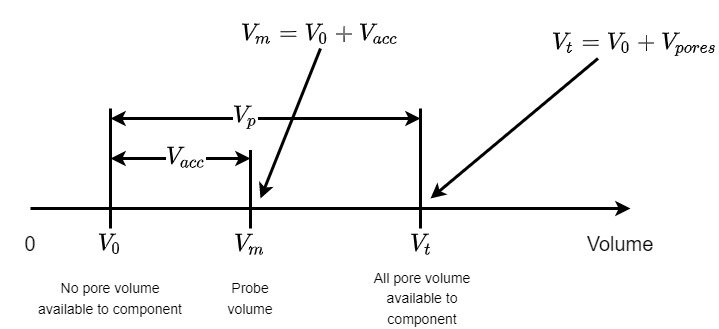
\includegraphics[width=0.7\textwidth]{SEC_volume.jpg}
    \caption{Schematic picture of different void volumes with respect to the
    molecule's elution volume. $V_0$ represents the column's extra (inter-)
    particle void volume. $V_t$ is the total void volume; i. e., $V_0$ and void
    volume inside all pores of all particles. The difference $V_t - V_0$ is
    volume of all pores inside all beads. $V_acc(r_m)$ is the sum of all pore
    volumes that are accessible to specific probe molecule of radius $r_m$.}
	\label{fig:volScale}
\end{figure}

Since probe molecule has a finite size and the pores sizes range from $r_{min}$
to $r_{max}$ not all pores' void volume is available to the molecule. The
accumulative volume of all pores that can be permeated by a molecule of size
$r_m$ is designated by $V_{acc}(r_m)$. 

By definition we know that $V_{acc}(r_m)$ is in the interval $[V_0, V_t]$.
Lower bound means that molecules can't fit into any of the pores, while upper
limit corresponds to a case where molecule's size allows for penetration of all
present pores, see figure \ref{fig:volScale}.

In order to quantify this phenomena new quantity is introduced, ratio between
accumulative accessible pore volume and all present pore volume, $K$:

\begin{equation}\label{eq:exclusion_factor}
    K(r_m) = \frac{V_{acc}(r_m)}{V_p}
\end{equation}

Newly introduced quantity is called exclusion factor and it represents fraction 
of the total pore volume of the matrix which is accessible to a molecule of 
radius $r_m$.

\begin{figure}[h]
	\centering
    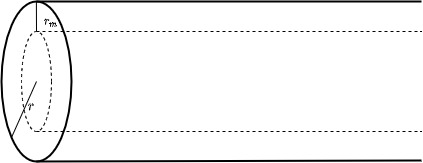
\includegraphics[width=0.4\textwidth]{probe_accessible_vol.jpg}
    \caption{$V_0$ is the column void volume available to all molecules
    (including very large ones). $V_t$ is the total void volume which is $V_0$
    and all void volume in bead's pores. Molecule which can fit into some}
	\label{fig1}
\end{figure}

Let us now focus only on one pore size. Accessible volume for spherical probe 
molecule with radius, $r_m$ and infinite cylindrically shaped pore with radius
$r$ is:
\begin{equation} \label{eq:acc_vol}
    V_{acc}(r, r_m) = \pi (r - r_m )^2 * L
\end{equation}
and whole volume of corresponding pore:
\begin{equation}
    V_{p}(r) = \pi r^2 * L,
\end{equation}
where $L\rightarrow\infty$. An important assumption is that we model pores by 
infinitely long cylinders.


Now we can define the $V_{acc}$ as pore volume that is accessible to all probe
molecules. Local exclusion factor $K(r, r_m)$ is:
\begin{equation}
    K(r, r_m) = \frac{V_{acc}}{V_{pore}} = \frac{\pi (r-r_m)^2 L}{\pi r^2 L} = \left(1 -
    \frac{r_m}{r}\right)^2
\end{equation}

To be more accurate, we should take into account, that pore radius might be smaller
than the probe size. In this case accessible volume for specific probe pore
combination is zero. We get following expression for the local exclusion
factor:
\begin{equation}\label{eq:local_ex_coeff}
	K(r, r_m) = 
	\begin{cases}
        \left(1 - \frac{r_m}{r}\right)^2 & r_m < r,  \\
		0           & r_m \geq r
	\end{cases}
\end{equation}


In reality the chromatographic column contains beads with pores of many
different sizes. In order to account for this, we use a distribution function
$f(r)$ which describes how pore volume is distributed across the pore sizes $r$.
By definition the $f(r)\ud r$ is the pore volume of pores that have radius $r$.
Thus, the integral from $r_1$ to $r_2$ is a pore volume of all pores that have
radius between $r_1$ and $r_2$:

\begin{equation}
    V_p(r_1 < r < r_2) = \int_{r_1}^{r_2}f(r)\ud r
\end{equation}

At this point we should mention one important distinction. Two volumes, total
pore volume and total accessible pore volume for smallest available probe
molecule. As smallest available probe molecule is usually very small, both 
volumes are very close to each other.
However, they are not the same. In some articles total accessible volume is used
for normalization, while in some other cases the total pore volume is used for
the normalization. If we define both volumes with convenient equation we get
following expressions:
\begin{equation}\label{eq:normalization}
    V_{p_{total}} = \int_{-\infty}^{\infty}f(r)\ud r
\end{equation}
in contrast to:
\begin{equation}\label{eq:alt_normalization}
    V_{p_{total\_acc}} =
    \int_{r_{min}}^{\infty}\left(1-\frac{r_{min}}{r}\right)^2f(r)\ud r
\end{equation}
By the definition of exclusion factor proper normalization would be equation
\ref{eq:normalization}. It is important to note, that we will use it in further
calculations, but equivalent exclusion factor model would be achieved if we
would decide for normalization with expression \ref{eq:alt_normalization}.

The pore distribution function $f(r)$ is not , but according to FABI and
Philips REF, best results are achieved by utilizing the log-distribution function

\begin{equation}
    f(r) = TODO
\end{equation}

If $f(r)$ is the volume fraction of pores of radius $r$, then the exclusion
coefficient for a molecule of radius $r_m$ is given by:

Derivation:
For cylinders with radius $r$ the available (not accessible) volume is
\begin{equation}
    V_p(r) = V_pf(r)
\end{equation}

In order to get accessible volume for a  molecule of $r_m$ we have to multiply
equation \ref{eq:local_ex_coeff} by the available volume:

\begin{equation}
    V_{acc}(r_m, r) = V_p(r) K(r_m, r) = V_p f(r) \left(1-\frac{r}{r_m}\right)^2
\end{equation}

Then the total accessible volume for molecule of size $r_m$ is:
\begin{equation}
    V_{acc}(r_m) = \sum_{r=r_m}^{r=\infty} V_p f(r)
    \left(1-\frac{r}{r_m}\right)^2,
\end{equation}

and in continuous case, we replace sum with an integral and distribution with a
differential distribution:
\begin{equation}
    V_{acc}(r_m) = \int_{r_m}^{\infty} V_p f'(r)
    \left(1-\frac{r}{r_m}\right)^2\ud r
\end{equation}

and in the end dividing $V_{acc}(r_m)$ by total pore volume $V_p$ we get final
equation for exclusion coefficient:
\begin{equation}
    K = \sum_{r = r_m}^{r = \infty} f(r)\left(1 - \frac{r}{r_m}\right)^2
\end{equation}

or in continuous case where $f'(r)\ud r$ represents the fraction of pore volume
within a range $r$ to $r+\ud r$ and is given by
\begin{equation}
    K = \int_{r_m}^{\infty} f'(r)\left(1 - \frac{r}{r_m}\right)^2\ud r
\end{equation}




\appendix

\section{Glossary}

Here one may find few common but also prone to raise a confusion terms, which
are grouped together in a meaningful way  order to elevate understanding and 
memorization of those.


Some commonly used Latin prefixes:
\begin{itemize}
    \item \textbf{extra-} or \textbf{extro-} - outside (slo. zunaj) - extra-particle volume
    \item \textbf{inter-} - between or among (slo. med) - inter-particle volume,
        inter-molecular bonds.
    \item \textbf{intra-} - within (slo. znotraj) - intra-particle volume,
        intra-molecular bonds.
\end{itemize}


